\documentclass{beamer}

\usepackage[utf8]{inputenc}
\usepackage{pdfpages}
\usepackage{listings}


%Information to be included in the title page:
\title{Foreman Provisioning}
\author{Emerson Ford}
\date{}



\begin{document}
\frame{\titlepage}

\begin{frame}
	\frametitle{SLATE Provisioning Goals}
	SLATE wants to provisions hosts across the world. How can we best do this?
	\begin{itemize}
		\item Plug into existing infrastructure
		\item Solution should be adaptable to a variety of scenarios
		      \begin{itemize}
			      \item No network configuration access
			      \item Have network configuration access
		      \end{itemize}
		\item Majority of work is pushed to us, not to staff at remote site
		\item Allow for automation of the majority of provisioning
		\item Centralized reporting of hosts
		\item Scalable, both with the number of hosts and distances between hosts
		\item Could potentially plug into other cloud providers.
	\end{itemize}
\end{frame}

\begin{frame}[fragile]
	\frametitle{Overview of Provisioning}
	\begin{columns}
		\begin{column}{0.5\textwidth}
			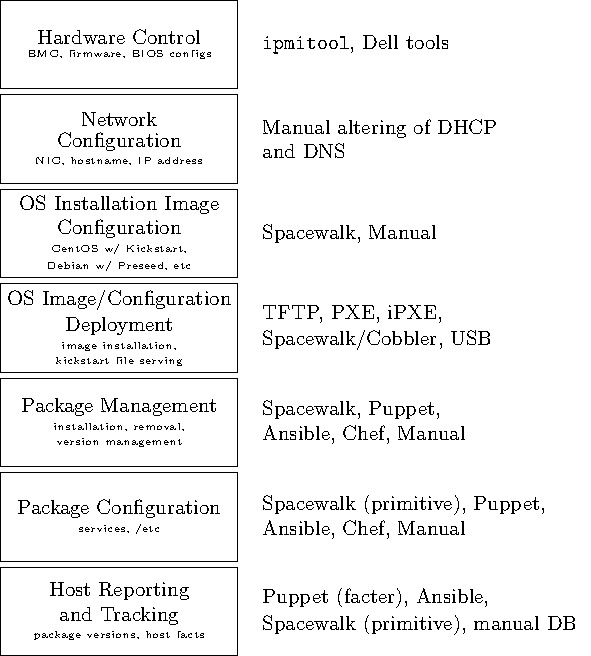
\includegraphics[width=\textwidth,height=\textheight-15mm,keepaspectratio]{provisioning_diagram}
		\end{column}

		\begin{column}{0.5\textwidth}
			Provisioning new machines is complicated... at the CHPC we have the following options:
			\begin{itemize}
				\item Can do all of this manually.
				\item Use Spacewalk, configure the rest manually.
				\item Configure hardware control \& network configuration manually, use one image/directory (through NFS) for all nodes (our compute nodes)
			\end{itemize}
			These aren't really scalable...
		\end{column}
	\end{columns}
\end{frame}

\begin{frame}
	\frametitle{What is Foreman?}
	An open-source project that acts as the "glue" between all of these pieces required for provisioning.
	It is extremely modular and plugs into existing projects like Puppet, xinetd, Kickstart, etc.
\end{frame}

\begin{frame}
	\frametitle{Foreman Architecture Overview}
	\centering
	\begin{figure}[t]
		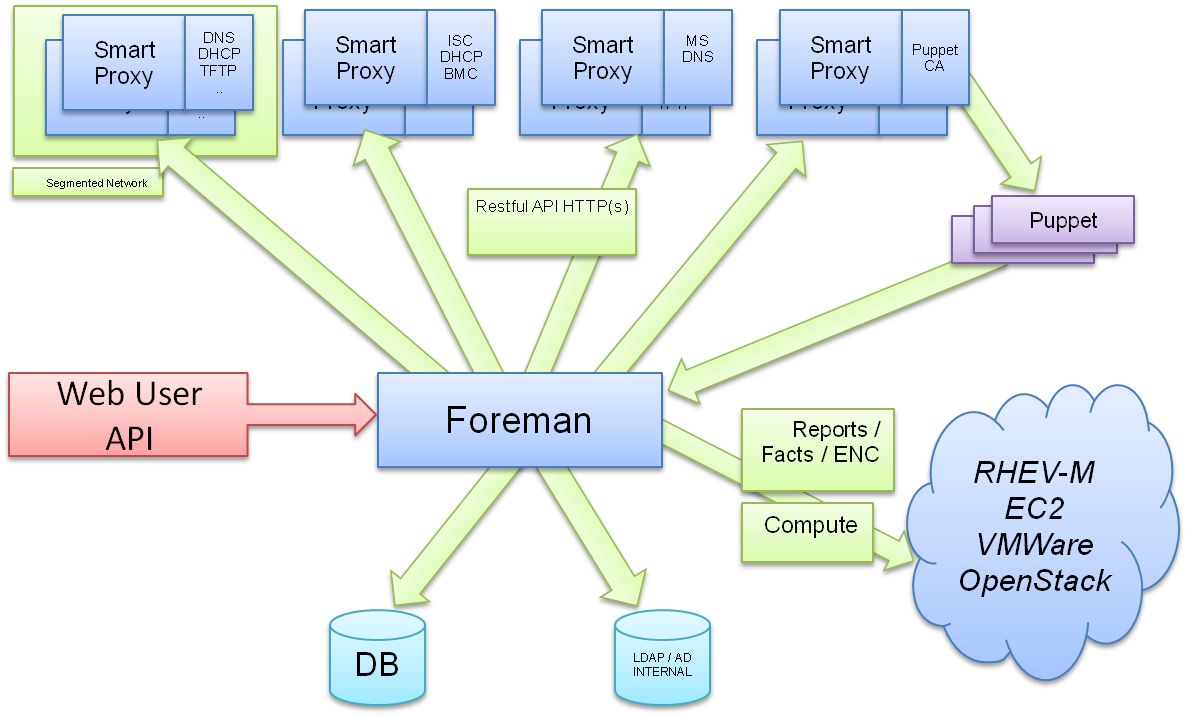
\includegraphics[width=\textwidth,height=\textheight-4cm,keepaspectratio]{foreman_architecture}

		\tiny Credit: Foreman Manual
	\end{figure}
	Each piece of Foreman can be deployed on individual servers. Smart Proxies plug into existing services, such as an already running \texttt{tftpd}.
\end{frame}

\begin{frame}[fragile]
	\frametitle{How Foreman Plugs into the Provisioning Stack}
	\begin{center}
		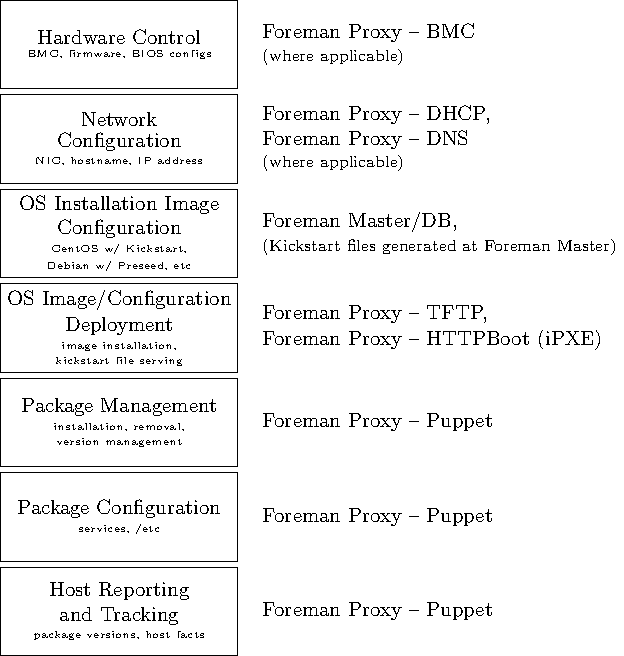
\includegraphics[width=\textwidth,height=\textheight-15mm,keepaspectratio]{provisioning_foreman_diagram}
	\end{center}
\end{frame}


\begin{frame}
	\frametitle{Foreman Overview -- Web/CLI}

	\begin{figure}[t]
		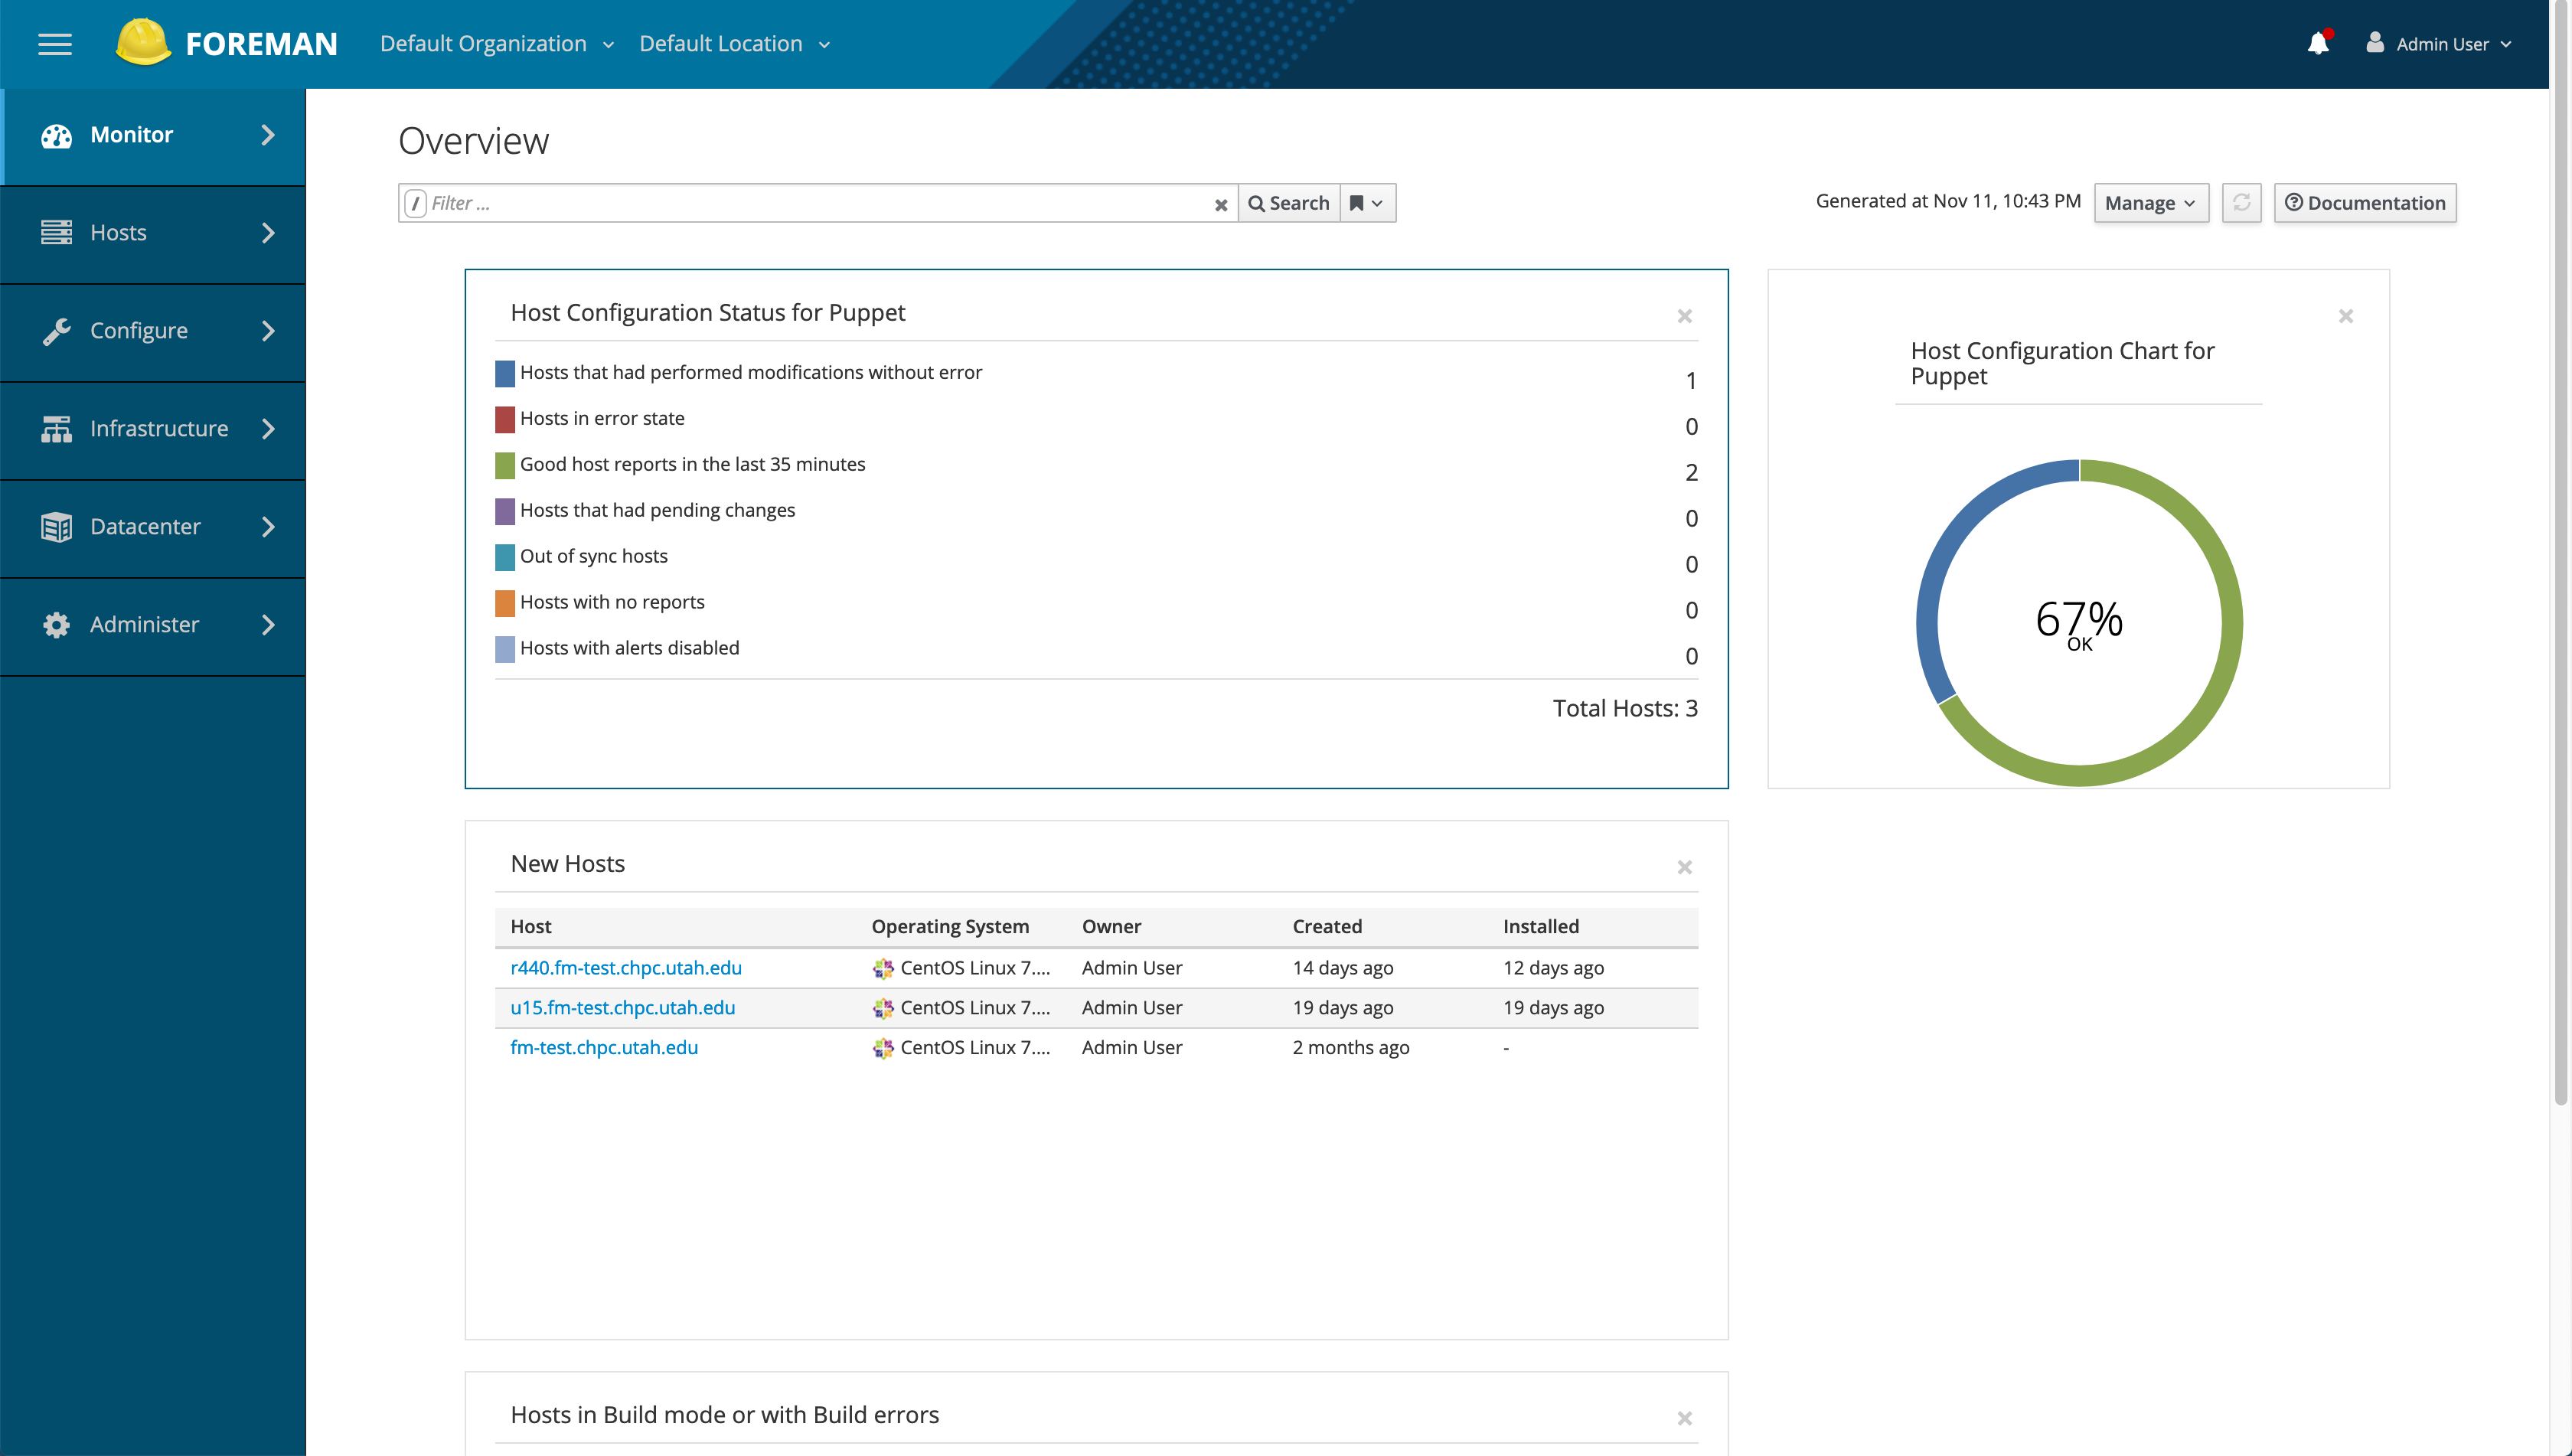
\includegraphics[width=\textwidth,height=\textheight-3cm,keepaspectratio]{foreman-web}
	\end{figure}

	Management of all provisioning pieces can be done through the Foreman web interface or Foreman CLI (\texttt{hammer}).


\end{frame}

\begin{frame}
	\frametitle{Other Benefits of Foreman}
	\begin{itemize}
		\item Extensive plugin ecosystem
		      \begin{itemize}
			      \item \textbf{Datacenter} provides capability to store physical DC information like rack location, power connection, switch connection, etc per host.
			      \item \textbf{Ansible} provides integration with Ansible.
			      \item \textbf{Discovery} provides MaaS capability.
			      \item \textbf{Katello} provides package versioning/repo management.
		      \end{itemize}
		\item Provides audit history of all configuration changes.
		\item Has integrations for GCE, AWS, Azure, Libvirt, OpenStack, VMWare, etc. Can use the same configurations for bare-metal, VM, or cloud VMs.
		\item Can store configurations as "profiles" and dynamically rebuild hosts with new profiles.
	\end{itemize}
\end{frame}

\begin{frame}
	\frametitle{Adding New Hosts to Foreman}
	There are two ways to add hosts:
	\begin{enumerate}
		\item Go through discovery workflow
		      \begin{itemize}
			      \item Provides MaaS functionality
			      \item Remote sites just need to plug in a USB and provide DHCP and we can take it from there
			      \item Host first boots into "Discovery" image and registers with Foreman as a "discovered host."
			      \item Then add this "discovered host"'s host entry to Foreman either through user button-click approval or automatic regex match.
		      \end{itemize}
		\item Manually register host in Foreman with the host's MAC address
		      \begin{itemize}
			      \item Host immediately boots into configured image and configurations.
			      \item Skips Discovery image workflow
		      \end{itemize}
	\end{enumerate}
	Both of these can route our custom iPXE image workflow.
\end{frame}

\begin{frame}[fragile,t]
	\frametitle{Custom iPXE Image}
	\flushleft
	Near vanilla iPXE image with the following embedded script:

	\centering
	\begin{lstlisting}[language=bash,frame=single,basicstyle=\fontsize{3.5}{5pt}\selectfont]
#!ipxe
:net0
isset ${net0/mac} || goto no_nic
dhcp net0 || goto net1
chain http://fm-test.chpc.utah.edu/unattended/iPXE?mac=${net0/mac} || goto net1

:net1
isset ${net1/mac} || goto no_nic
dhcp net1 || goto net2
chain http://fm-test.chpc.utah.edu/unattended/iPXE?mac=${net1/mac} || goto net2
...
:no_nic
echo Failed to chainload from any network interface
sleep 30
exit 1
  \end{lstlisting}
	Boot into Custom iPXE Image can happen in two ways:
	\begin{enumerate}
		\item USB boot with custom iPXE image.
		\item PXE boot into custom iPXE image (configure DHCP):
	\end{enumerate}
	\begin{lstlisting}[frame=single,basicstyle=\fontsize{3.5}{5pt}\selectfont]
if exists user-class and option user-class = "iPXE" {
  filename "http://fm-test.chpc.utah.edu/unattended/iPXE?bootstrap=1";
} elsif option architecture = 00:06 {
  filename "ipxe.efi";
} 
...
else {
  filename "undionly.0";
}
          \end{lstlisting}

\end{frame}

\begin{frame}[fragile]
	\frametitle{Foreman Discovery Workflow}

	\begin{columns}
		\begin{column}{0.5\textwidth}
			\flushleft
			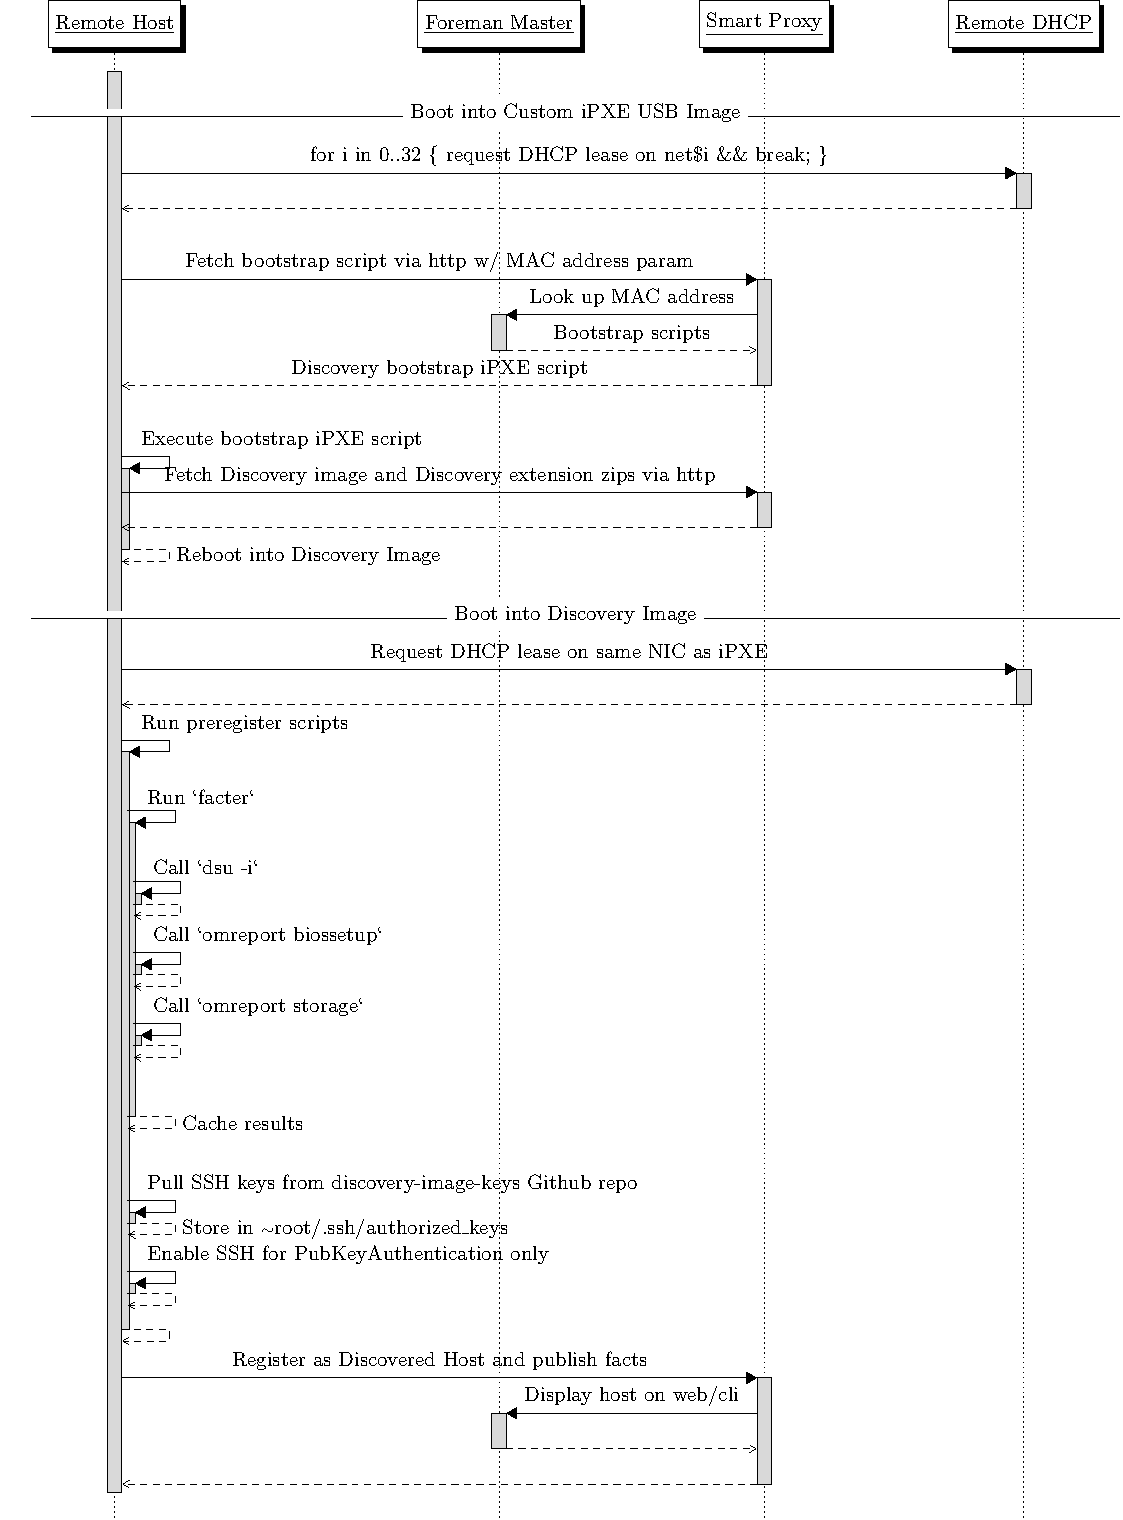
\includegraphics[width=\textwidth,height=\textheight-15mm,keepaspectratio]{discovery_sd}
		\end{column}

		\begin{column}{0.5\textwidth}
			\small
			Host entry not found $\Rightarrow$ discovery workflow

			Host entry found $\Rightarrow$ skip to installation workflow
			\vspace{.5cm}

			Custom things added to Discovery image:
			\begin{enumerate}
				\item OMSA and DSU tools/Facter facts
				\item Pulls SSH keys from discovery-image-keys.git
				\item Enable SSH only for PubkeyAuthentication
			\end{enumerate}

			SLATE admins currently need to manually SSH in to configure BIOS/firmware before provisioning. Looking to automate this.

		\end{column}
	\end{columns}
\end{frame}

\begin{frame}[fragile]
	\frametitle{Foreman Installation Workflow}

	\centering
	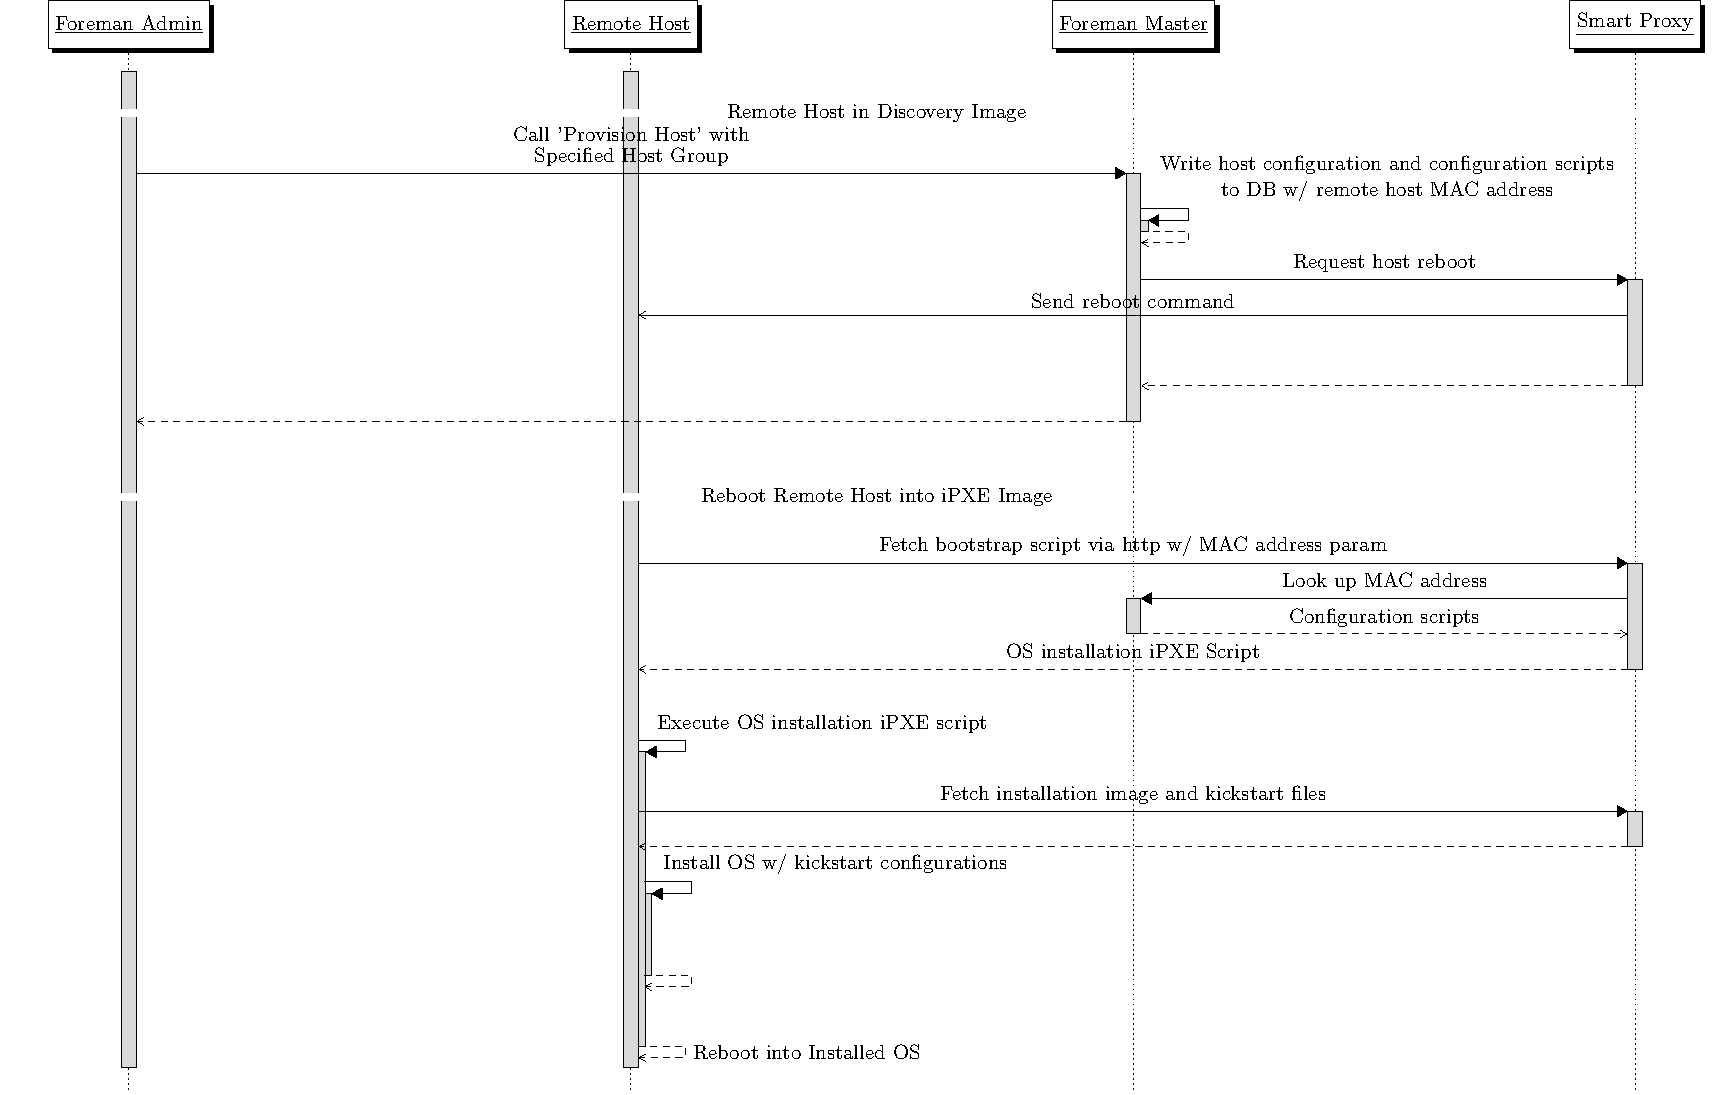
\includegraphics[width=\textwidth,height=\textheight-35mm,keepaspectratio]{installation_sd}

	\tiny Foreman supports kickstart files (RedHat), preseed files (Debian), etc.
	\vspace{.5cm}

	\normalsize Provision host can be automatic with regex match rules (ie. if host has model type, automatically provision with this profile).
\end{frame}

\begin{frame}[fragile]
	\frametitle{Foreman Configuration Workflow}

	\centering
	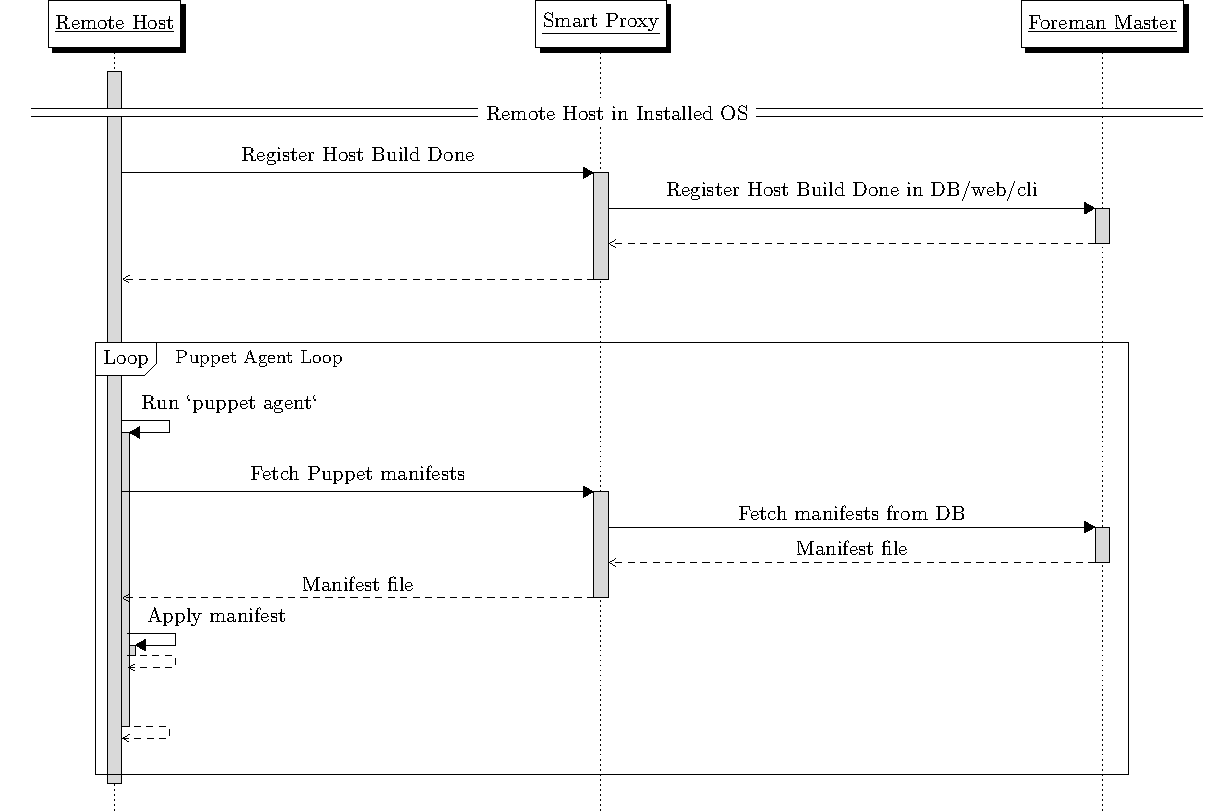
\includegraphics[width=\textwidth,height=\textheight-35mm,keepaspectratio]{configuration_sd}

	\tiny Foreman comes with Puppet by default but can be configured with Ansible, SaltStack, etc.
	\vspace{.5cm}

	\normalsize Puppet can be used both normally (ie. with manifests) or Puppet class configurations can be done through Foreman.
\end{frame}

\begin{frame}
	\frametitle{Current Status}
	\begin{enumerate}
		\item Old OOB box (R440) has gone through this full workflow, currently managed with SLATE Puppet scripts.
		      \begin{itemize}
			      \item Done with a USB to show it works without DHCP configuration access.
		      \end{itemize}
		\item Was able to update firmware with \texttt{dsu} in Discovery Image manually.
		\item Was able to make BIOS change with \texttt{omconfig} in Discovery Image manually.
		\item BIOS configurations are reported in Facter/Foreman Web UI, including when the host is in the "Discovered" stage.
		      \begin{itemize}
			      \item \texttt{dsu} output is still a WIP.
		      \end{itemize}
		\item Looking to modify the dell-ansible module to automate BIOS changes and firmware updates.
	\end{enumerate}

\end{frame}
\end{document}
